
\lecture{Dependent Populations}{dependent-populations}
\section{Dependent Populations}

\title{Two Populations}
\subtitle{Dependent Populations}

%\author{Kelly Black}
%\institute{Clarkson University}
\date{6 April 2012}

\begin{frame}
  \titlepage
\end{frame}

\begin{frame}
  \frametitle{Outline}
  \tableofcontents[hideothersubsections,sectionstyle=show/hide]
\end{frame}

\subsection{Clicker Quiz}

\begin{frame}{Clicker Quiz}

  \iftoggle{clicker}{%

    An advertisement includes a claim that ten percent of all people
    use a particular brand of toilet paper. I think that it should be
    more than that. I poll nine-hundred and fifty-six people and ask
    them if they use this brand of toilet paper. One-hundred and ten
    say yes. Is the claim true? (Use a five percent significant
    level.)

    \vfill 


    \begin{tabular}{l@{\hspace{3em}}l@{\hspace{3em}}l@{\hspace{3em}}l}
      A: Reject $H_o$.  & Do not reject $H_0$.
    \end{tabular}

    \vfill
    \vfill
    \vfill

  }

\end{frame}


\begin{frame}
  \frametitle{Comparison}

  \begin{columns}
    \column{0.33\textwidth}
    Normal Distribution:
    \begin{eqnarray*}
      z &  = & \frac{\bar{x}-\mu}{\lp \frac{\sigma}{\sqrt{n}} \rp}.
    \end{eqnarray*}

    \column{0.33\textwidth}
    $t$-Distribution:
    \begin{eqnarray*}
      t &  = & \frac{\bar{x}-\mu}{\lp \frac{s}{\sqrt{n}} \rp}, \\
      df & = & n-1.
    \end{eqnarray*}

    \column{0.33\textwidth}
    Proportions:
    \begin{eqnarray*}
      z & = & \frac{\hat{p}-p}{\sqrt{\frac{p(1-p)}{n}}},
    \end{eqnarray*}


  \end{columns}

  \vfill

    \only<2->
    {
      \begin{center}
        The algebra and concepts are exactly the same!
      \end{center}
    }

    \vfill
  

\end{frame}


\subsection{Multiple Samples}


\begin{frame}
  \frametitle{Example}

  I pick a random sample of one-hundred stocks and calculate their
  predicted values in one year using a model. I then pick a random
  sample of one-hundred and ten stocks and get their predicted values
  in one year using a different model. Is there a difference in the
  mean stock price after one year between the two models?

  \uncover<2->
  {
    \begin{columns}
      \column{.5\textwidth}
      \begin{tabular}{l}
        Group 1 \\ \hline
        $N_1=100$, \\
        $\bar{x}$, \\
        $s_x$
      \end{tabular}

      \column{.5\textwidth}
      \begin{tabular}{l}
        Group 2 \\ \hline
        $N_2=110$, \\
        $\bar{y}$, \\
        $s_y$
      \end{tabular}

    \end{columns}
  }

  \uncover<3->
  {
    Independent Samples!
  }

  \hfill

\end{frame}


\begin{frame}
  \frametitle{Example}

  I pick a random sample of one-hundred stocks and calculate their
  predicted values in one year using a model. I then wait a year and
  get their actual values. Is there a difference in the mean predicted
  prices and the actual prices?

  \uncover<2->
  {
    \begin{columns}
      \column{.5\textwidth}
      \begin{tabular}{l}
        Group 1 Predicted \\ \hline
        $N=100$, \\
        Predicted Price
      \end{tabular}

      \column{.5\textwidth}
      \begin{tabular}{l}
        Group 1 Actual \\ \hline
        $N=100$, \\
        Actual Price
      \end{tabular}

    \end{columns}
  }

  \uncover<3->
  {
    Dependent Samples!
  }

  \hfill

\end{frame}



\begin{frame}
  \frametitle{Great, more stuff?}
  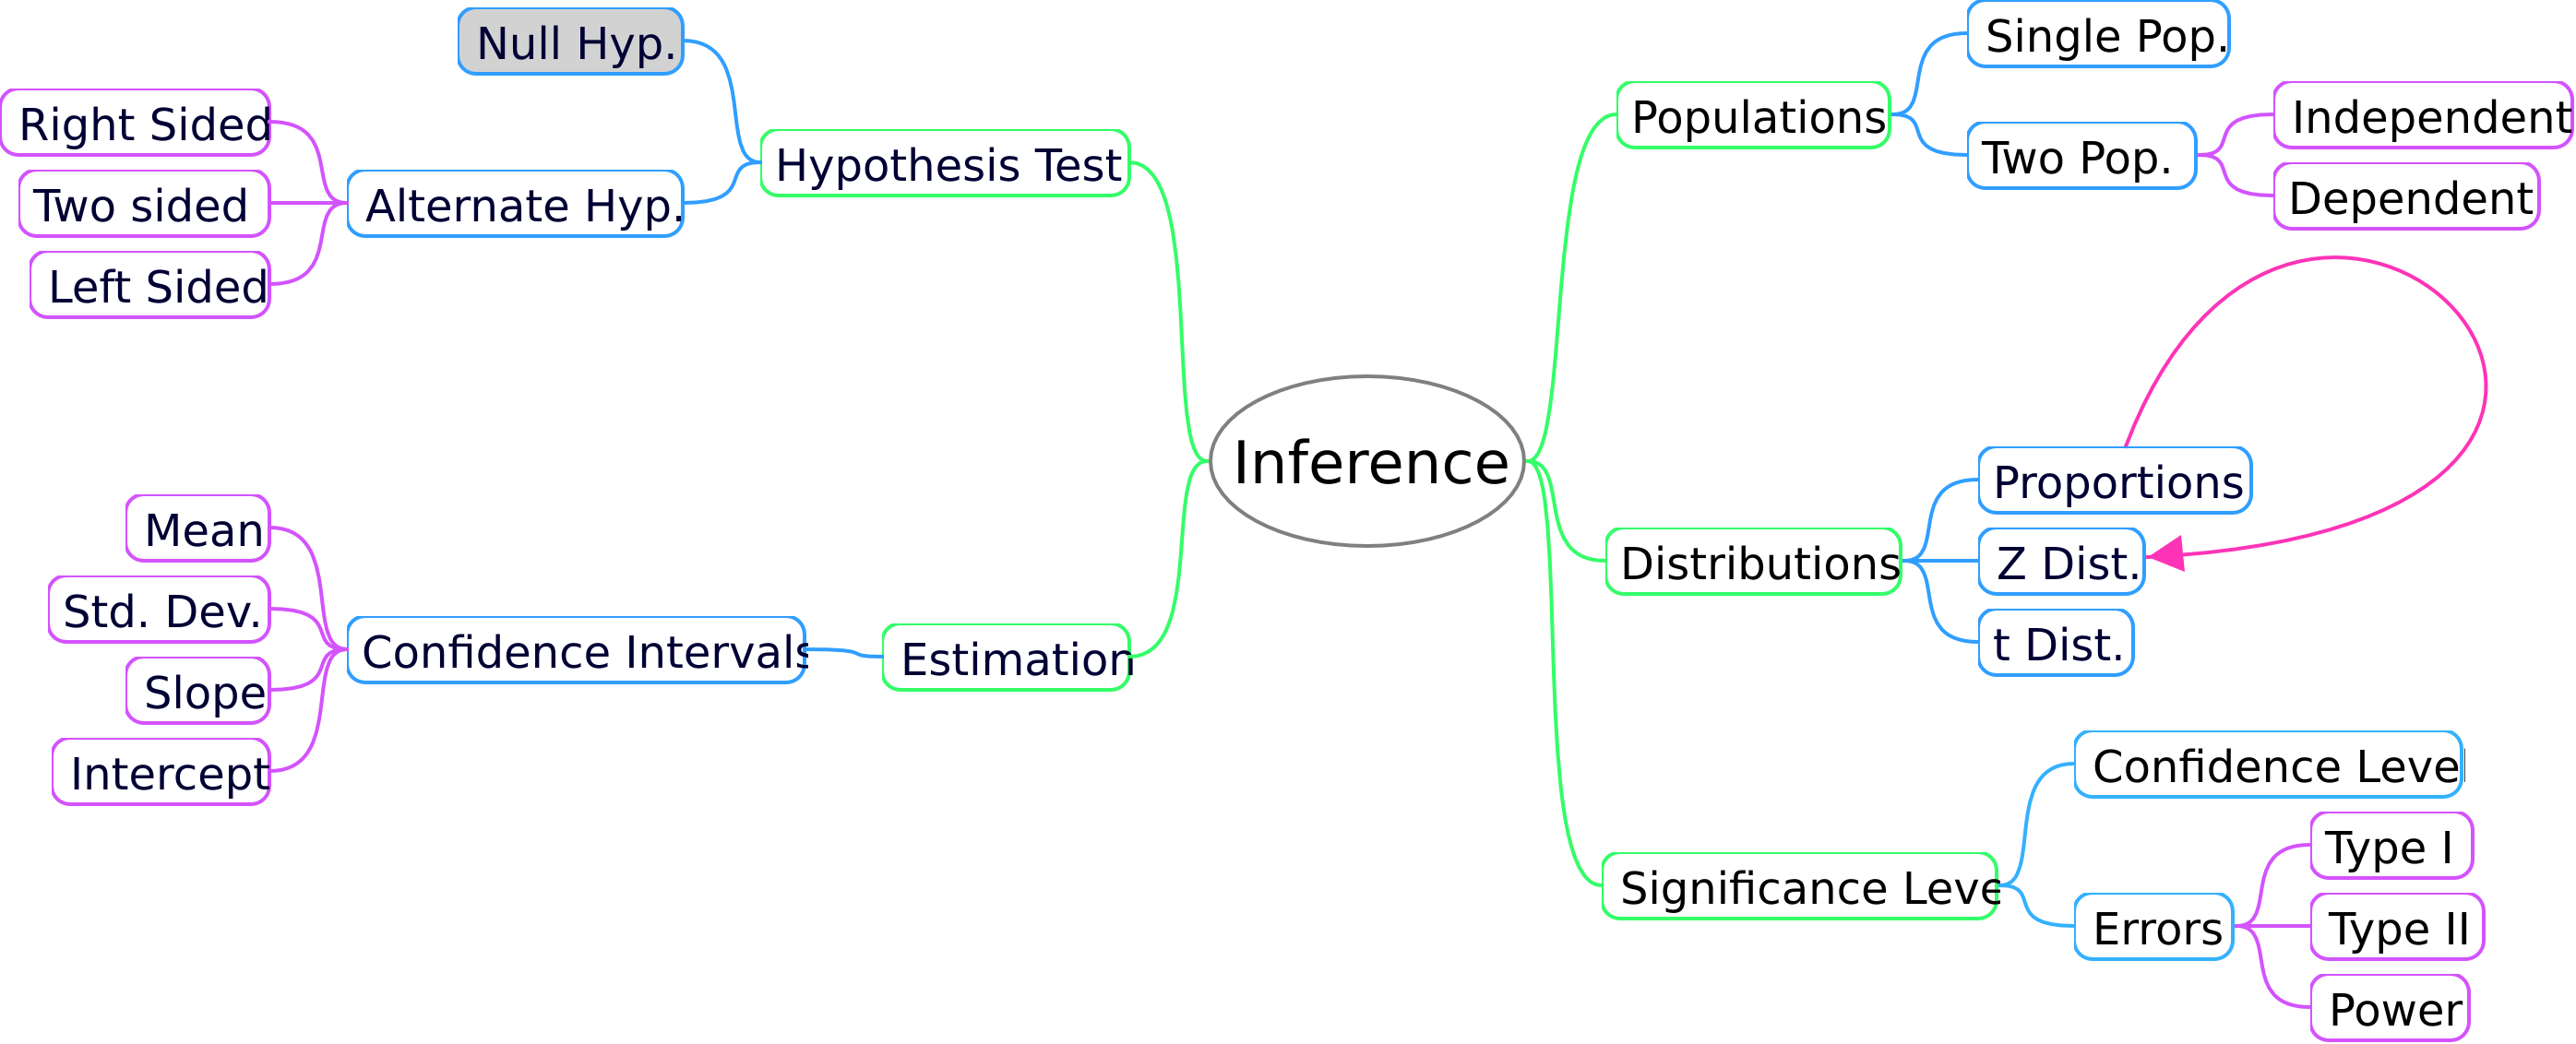
\includegraphics[width=8.5cm]{img/inference}
\end{frame}


\subsection{Dependent Populations}

\begin{frame}
  \frametitle{Dependent Populations}
% $\RightArrow$ {\onslide<2->}

  \only<3->{We can calculate a set of \textit{paired differences.}}
  \begin{tabular}{l<{\onslide<2->}l<{\onslide<3->}ll<{\onslide}l}
    Before & After & & Difference \\
    $x_1$ & $y_1$ & $\Rightarrow$ & $x_1-y_1$ \\
    $x_2$ & $y_2$ & $\Rightarrow$ & $x_2-y_2$ \\
    $x_3$ & $y_3$ & $\Rightarrow$ & $x_3-y_3$ \\
    $x_4$ & $y_4$ & $\Rightarrow$ & $x_4-y_4$ \\
    $\vdots$ & $\vdots$ & & $\vdots$ \\
    $x_n$ & $y_n$ & $\Rightarrow$ & $x_n-y_n$ \\
  \end{tabular}

\end{frame}


\begin{frame}{Another View}

  You have a set of ``before'' data:
  \begin{eqnarray*}
    \begin{array}{lllll}
      x_1 & x_2 & x_3 & \cdots & x_n
    \end{array}
  \end{eqnarray*}

  \only<2->
  {
    You have a set of ``after'' data:
    \begin{eqnarray*}
      \begin{array}{lllll}
        y_1 & y_2 & y_3 & \cdots & y_n
      \end{array}
    \end{eqnarray*}
  }

  \only<3->
  {
    You calculate a difference:
    \begin{eqnarray*}
      \begin{array}{lllll}
        w_1=x_1-y_1 & w_2=x_2-y_2 & w_3=x_3-y_3 & \cdots & w_n=x_n-y_n
      \end{array}
    \end{eqnarray*}
  }

  \only<4->
  {
    You can now calculate $\bar{w}$, $s_w$, $n$ and perform your
    confidence interval/hypothesis test just as before.
  }
    

  \vfill

\end{frame}

\begin{frame}{Clicker Quiz}

  \iftoggle{clicker}{%

    A new drug is trialed to see if it can help reduce hair
    loss. Six people will try the drug. Before the trial begins the
    mean number of hairs per square centimeters are found. At the end
    of the trial the mean number of hairs per square centimeters are
    found for each person. What is the 95\% confidence interval for
    the change in hair density?

    \begin{tabular}{ll}
      Before & After \\
      181 & 187 \\
      182 & 194 \\
      171 & 178 \\
      195 & 191 \\
      192 & 186 \\
      183 & 181
    \end{tabular}

    \vfill 


    \begin{tabular}{l@{\hspace{3em}}l@{\hspace{3em}}l@{\hspace{3em}}l}
      A: between -7.9 and 3.6 & 
      B: between -8.4 and 4.1 & 
      C: between -9.7 and 5.4 & 
      D: between -10.4 and 6.1
    \end{tabular}

    \vfill
    \vfill
    \vfill

  }

\end{frame}

\begin{frame}{Clicker Quiz}

  \iftoggle{clicker}{%

    \begin{columns}
      \column{.25\textwidth}
      \begin{tabular}{lll}
        Before & After & Difference \\
        181 & 187 & -6 \\
        182 & 194 & -12 \\
        171 & 178 & -7 \\
        195 & 191 & 4 \\
        192 & 186 & 6 \\
        183 & 181 & 2
      \end{tabular}
      
      \column{.75\textwidth}

      \only<2-> {

        \begin{eqnarray*}
          n & = & 6, \\
          \bar{x} & \approx & -2.166667, \\
          s & \approx &  7.167054, \\
          \mathrm{df} & = & 5, \\
          t^* & \approx & 2.571.
        \end{eqnarray*}

      }


    \end{columns}

        Confidence interval:
        \begin{eqnarray*}
          \bar{x} \pm t^* \frac{s}{\sqrt{n}}
        \end{eqnarray*}



    \vfill
    

  }

\end{frame}



\begin{frame}{Clicker Quiz}

  \iftoggle{clicker}{%

    A new drug is trialed to see if it can help reduce hair
    loss. Six people will try the drug. Before the trial begins the
    mean number of hairs per square centimeters are found. At the end
    of the trial the mean number of hairs per square centimeters are
    found for each person. What is the 95\% confidence interval for
    the change in hair density?


    The 95\% confidence interval for the difference in hair density is
    between -9.7 and 5.4 hairs/cm\textsuperscript{2} assuming a
    $t$-distribution with 5 degrees of freedom.

    \vfill
    

  }

\end{frame}


\begin{frame}{Clicker Quiz}

  \iftoggle{clicker}{%

    A new drug is trialed to see if it can help reduce hair loss. Six
    people will try the drug. Before the trial begins the mean number
    of hairs per square centimeters are found. At the end of the trial
    the mean number of hairs per square centimeters are found for each
    person. Did the drug make a difference? (Use a 95\% confidence
    level.)

    \begin{tabular}{ll}
      Before & After \\
      181 & 187 \\
      182 & 194 \\
      171 & 178 \\
      195 & 191 \\
      192 & 186 \\
      183 & 181
    \end{tabular}

    \vfill 


    \begin{tabular}{l@{\hspace{3em}}l@{\hspace{3em}}l@{\hspace{3em}}l}
      A: reject $H_0$ & 
      B: cannot reject $H_0$
    \end{tabular}

    \vfill
    \vfill
    \vfill

  }

\end{frame}



% LocalWords:  Clarkson pausesection hideallsubsections df lllll lll
